\documentclass[fontset=windows]{article}
\usepackage[margin=1in]{geometry}%设置边距,符合Word设定
\usepackage{ctex}
\usepackage{amsmath, xparse}
\usepackage{amssymb}
\usepackage{setspace}
\usepackage{lipsum}
\usepackage{graphicx}%插入图片
\usepackage{multirow}%多列表格
\usepackage{subfigure}
\graphicspath{{Figures/}}%文章所用图片在当前目录下的 Figures目录
\usepackage{hyperref} % 对目录生成链接,注:该宏包可能与其他宏包冲突,故放在所有引用的宏包之后
\hypersetup{
    colorlinks        = true,  % 将链接文字带颜色
	bookmarksopen     = true, % 展开书签
	bookmarksnumbered = true, % 书签带章节编号
	pdftitle          = 标题, % 标题
	pdfauthor         = DarkSharpness, % 作者
    citecolor         = green,
    linkcolor         = black,
    urlcolor          = blue
}
\bibliographystyle{plain}% 参考文献引用格式
\newcommand{\upcite}[1]{\textsuperscript{\cite{#1}}}

\renewcommand{\contentsname}{\centerline{Contents}} %经过设置word格式后,将目录标题居中

% Keywords command
\providecommand{\keywords}[1]
{
  \textbf{\text{Keywords: }} #1
}

\title{\heiti\zihao{2} 抽水泵}
\date{2024.01.14}

\begin{document}
	\maketitle
	% \thispagestyle{empty}

\begin{abstract} 
    一个简单的水泵可以将一根吸管折成三角形,并在顶点处切开的方式来制作。当这样一个三角形部分浸入水中,其中一个顶点绕其三角形的竖直轴旋转时,水可能会通过吸管流向上方。我们对这一现象进行了理论解释,并设计实验与理论模型进行比对,实验结果证明了其合理性。
\end{abstract}

\tableofcontents

\newpage

\section{引言}

一个简单的水泵可以将一根吸管折成三角形,并在顶点处切开的方式来制作。当这样一个三角形部分浸入水中,其中一个顶点绕其三角形的竖直轴旋转时,水可能会通过吸管流向上方。

如图 $1$ 所示,我们用一个将上述的吸管三角形绑在一个木棒上,用来控制吸管的转动。将吸管下端部分浸入水中,并且快速的用手转动木棒,可以观察到水花被吸管从下面的水盆中抽出,四处飞溅。

\begin{figure}[htbp]
    \centering
    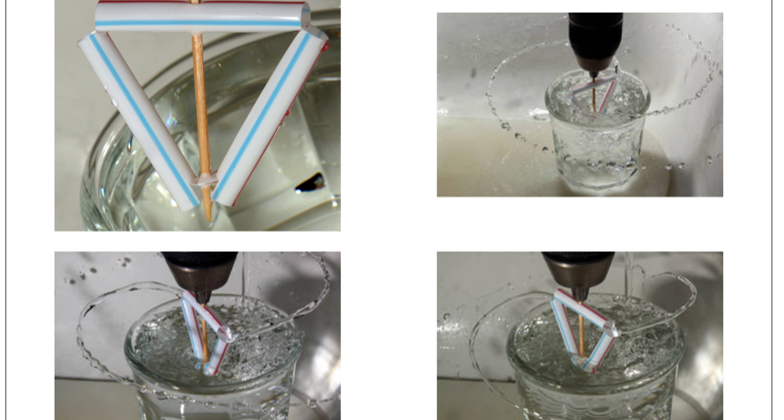
\includegraphics[scale=0.5]{7.png}
    \caption{实际效果图}
    \label{1}
\end{figure}


\section{理论模型}

我们假定吸管搭成的是一个等腰三角形,并且用一个长木棒穿过其顶点以及底边中点。我们将这个三角形的顶点一段置于水盆中,并且通过木棒来控制吸管使其绕着木棒旋转。

\begin{figure}[htbp]
    \centering
    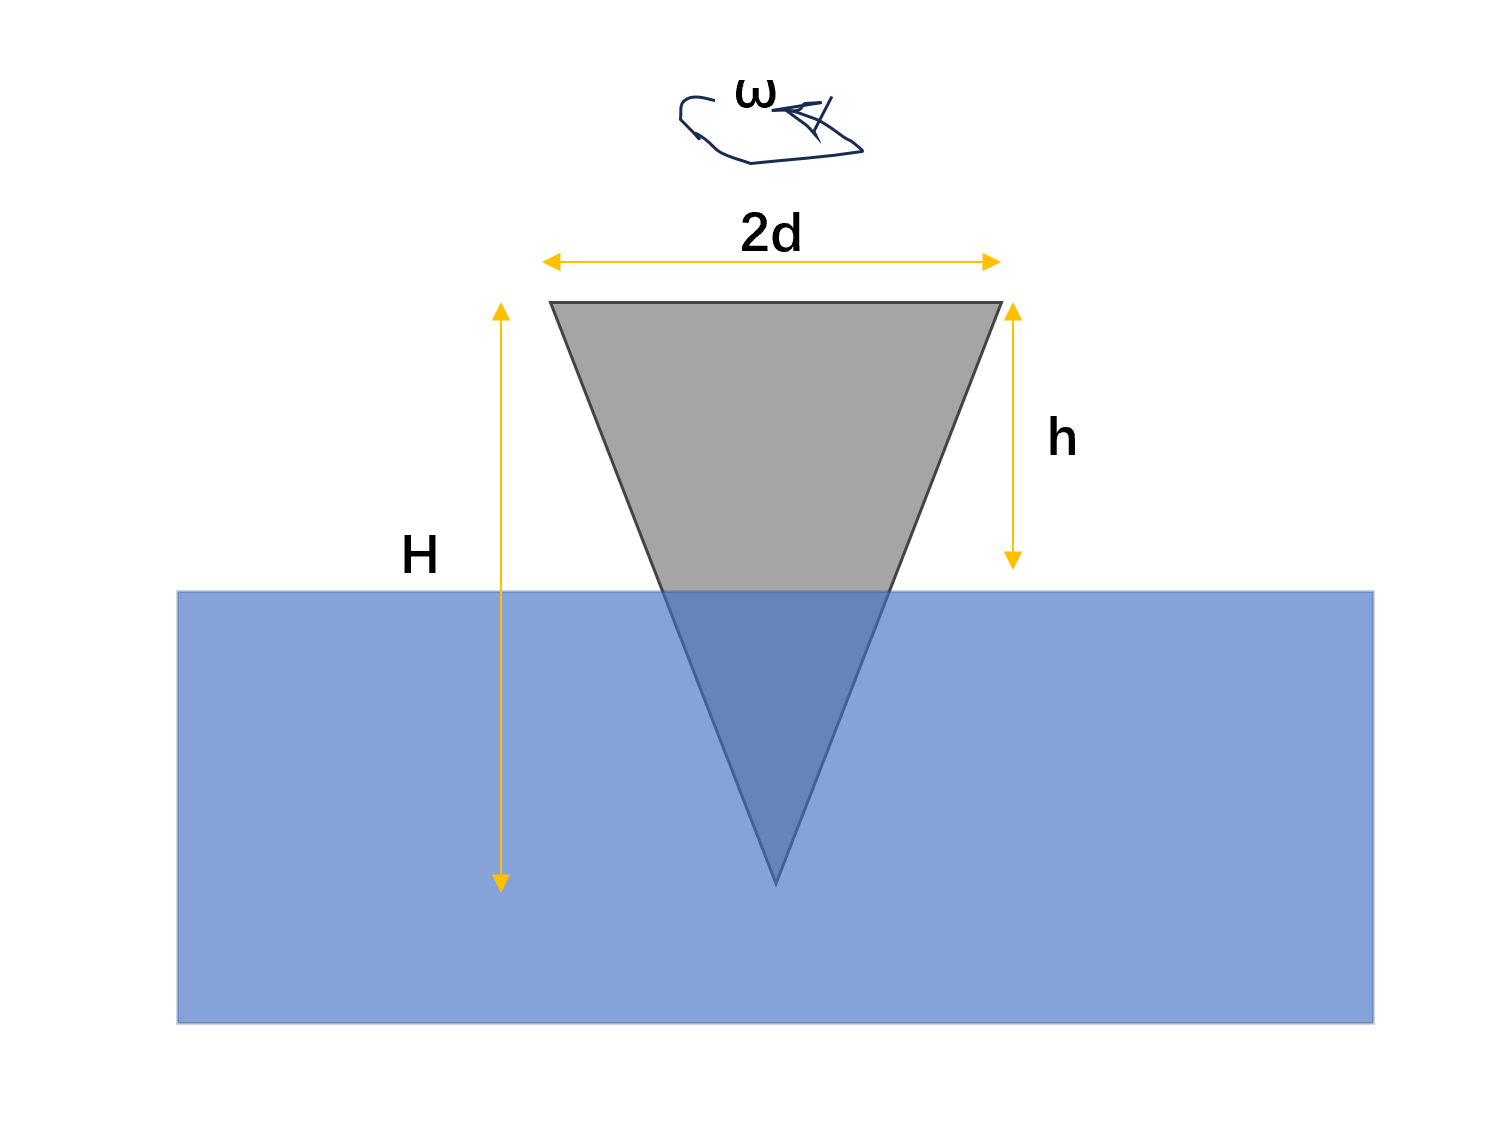
\includegraphics[scale=0.5]{8.png}
    \caption{几何参数示意图}
    \label{2}
\end{figure}

设等腰三角形的两条斜边长度为 $l$ ,且底边长度为 $2d$ ,露出水面部分的高度 (即水平面到底边的距离) 为 $h$。设木棒转动的角速度为 $\omega$ 。设重力加速度为 $g$ 。设吸管的横截面积为 $A$ ,且远小于水盆的面积。设大气压强为 $p_0$ 。由勾股定理,三角形的高为 $H = \sqrt{l ^ 2 - d ^ 2}$ 。

简单起见,我们假设木棒和吸管做匀速旋转。因此,水流在空间中特定一点的流速 (或者说速度场) 可以视作是不随时间变化的。同时,我们假设吸管内部水流近似均匀,且假设吸管的横截面积远小于水盆的面积。我们不考虑水与水之间以及水和吸管壁之间的粘滞阻力,认为水是不可压缩的理想流体。

\subsection{吸管内部}

由于吸管跟随木棒旋转,因此我们选择在旋转坐标系中进行力学分析。

基于我们的水流近似均匀的假设,以及流量守恒,我们可以假设吸管内部水流的沿着管道速度是处处相等的。设内部水流的沿管道速度为 $v_l$ 。

在旋转坐标系,我们分析距离木棒轴 $r$ 处的位置液体微元的受力情况。在内部,因为流速均匀分布,且不随时间变化。因此,可以认为液体微元处处受力平衡。基于水是无粘性可压缩流体的假设,我们可以使用不含粘性项的 $\text{N-S}$ 方程,即:

$$
\rho\frac{\text{d}v}{\text{d}t} = - \nabla p - \rho \nabla \phi
$$

其中, $\frac{\text{d}}{\text{d}t} = \frac{\partial}{\partial t} + (v \cdot \nabla)$ , $\phi$ 为单位体积的流体的势能 (这里只含重力势能,以及旋转坐标系中的惯性离心力势能) 。但由于在吸管中,我们假定流速均匀分布,且不随时间变化,因此等式左边两项均为 $0$ ,且由于假定水不可压缩,有 $\rho = \text{Constant}$ 。因此, $\nabla (p + \rho \phi) = 0$ 即 $p + \rho \phi = \text{Constant}$ 。

取木棒轴为离心势能零点,在距离轴 $r$ 处的位置,惯性离心势为 $-\frac{1}{2}\omega^2 r^2$ 。设相对水面高度为 $y$ ,则此处的单位势为 $\phi = gy - \frac{1}{2}\omega^2 r^2$ 。

在开放端(水流出射点,即三角形底边的顶点),水与大气直接接触,其压强为 $p_0$ ,且距离轴 $d$ ,相对水面的高度为 $h$ 。在水流进入端(即三角形的顶点),其距离轴为 $0$ ,相对水面高度为 $h - H < 0$ 。因此,带入公式,三角形顶点处的压强 $p$ 满足:

$$
\begin{aligned}
    p + \rho g (h - H) - 0 = p_0 + \rho g h - \frac{1}{2}\rho\omega^2 d^2
    \iff p = p_0 + \rho g H - \frac{1}{2}\rho\omega^2 d^2
\end{aligned}
$$

\subsection{吸管外部}

在吸管底部(即三角形顶点)处,已求出其压强为 $p_1 = p_0 + \rho g H - \frac{1}{2}\rho\omega^2 d^2$ 。在吸管外部,由于假定水近似没有粘性,因此可以忽略木棒和吸管转动给水流带来的旋转影响。由于假定了吸管的横截面积远小于水盆的面积,我们可以用如下方法进行近似估算: 假设吸管顶点处有一个点,其压强恒定为 $p_1$ 。求出稳定分布下水流的流速情况。

回到地面系中。同理,由不含粘性项的 $\text{N-S}$ 方程,有:

$$
\rho\frac{\text{d}v}{\text{d}t} = - \nabla p - \rho \nabla \phi
$$

由于不随时间变化即 $\frac{\partial}{\partial t} = 0$ ,因此有 $\frac{\text{d}}{\text{d}t} = \frac{\partial}{\partial t} + (v \cdot \nabla) = v \cdot \nabla$ 。带入:

$$
\rho (v \cdot \nabla) v = - \nabla p - \rho \nabla \phi
$$

又因为忽略了转动给水带来的影响,应当有 $\nabla \times v = 0$ 。因此,$(v \cdot \nabla) v = \frac{1}{2} \nabla (v^2) - v \times (\nabla \times v) = \frac{1}{2} \nabla (v^2)$ 。又因为水不可压缩,即 $\rho = \text {Constant}$ ,且此时,在地面系中,势能项只含重力势,即 $\phi = gy$。因此,可以得到:

$$
\begin{aligned}
    \nabla (\frac{1}{2} \rho v ^ 2 + \rho g y + p) &= 0 \\ 
    \iff \frac{1}{2} \rho v ^ 2 + \rho g y + p &= \text{Constant}
\end{aligned}
$$

即满足伯努利方程。其中,一个确定的边界为液体的表面。因为吸管横截面积远小于液面,因此可以认为液面几乎不变。即水平面满足 $p = p_0 , v = 0 , y = 0$ 。因此,带入吸管底部条件 $p = p_1, v = v_l, y = h - H$ ,可得:

$$
v_l = \sqrt{\frac{1}{2}\omega^2 d^2 - gh}
$$

其中, $v_l$ 为管道内液体沿管道的速度, $\omega$ 为旋转的角速度, $d$ 为三角形底边长度的一半, $g$ 为重力加速度, $h$ 为三角形底边相对水平面的高度。

\section{实验设计}

\subsection{实验设备}

吸管若干,长木棒若干,502 强力胶水,胶带,瓶盖(或其他障碍物),一大盆水,摄像机,尺子。

\begin{figure}[htbp]
    \centering
    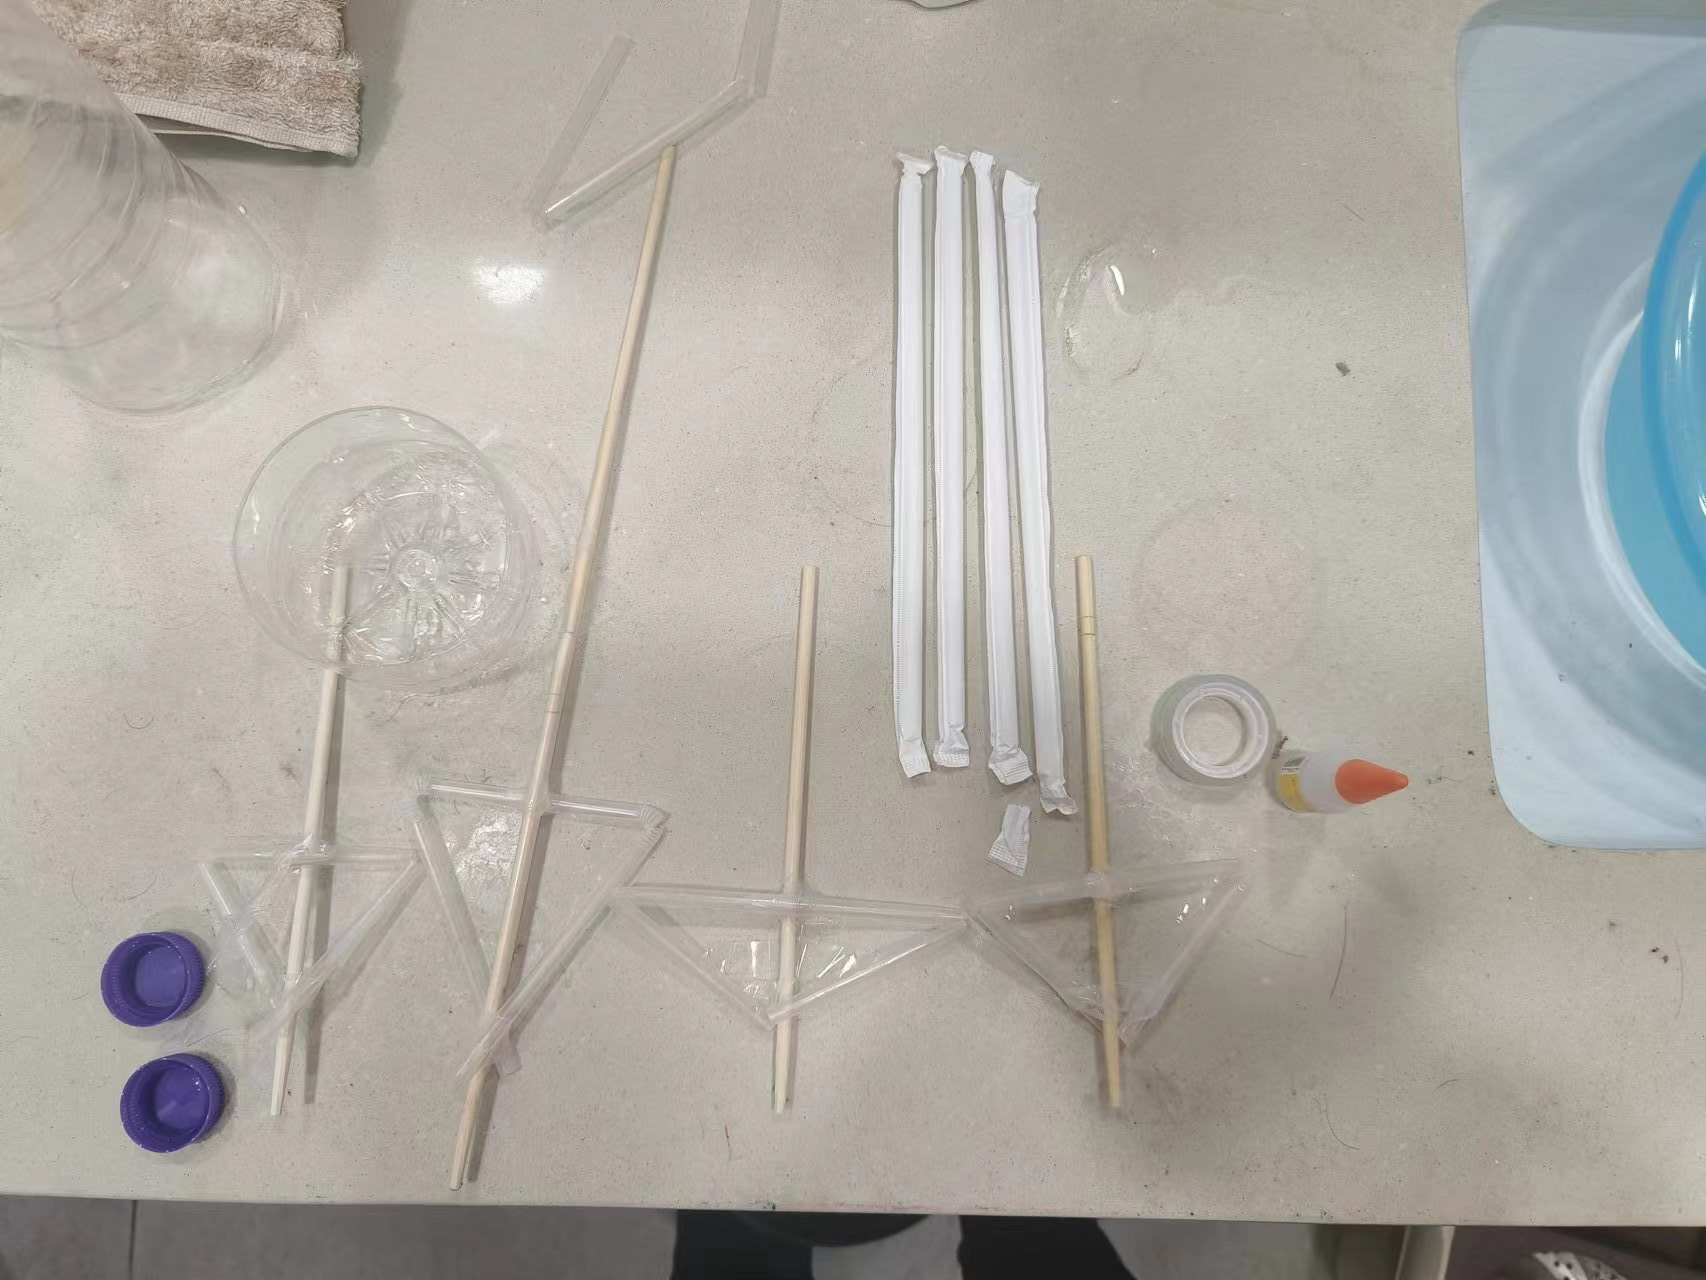
\includegraphics[scale=0.15]{10.png}
    \caption{仪器图}
    \label{3}
\end{figure}

\begin{figure}[htbp]
    \centering
    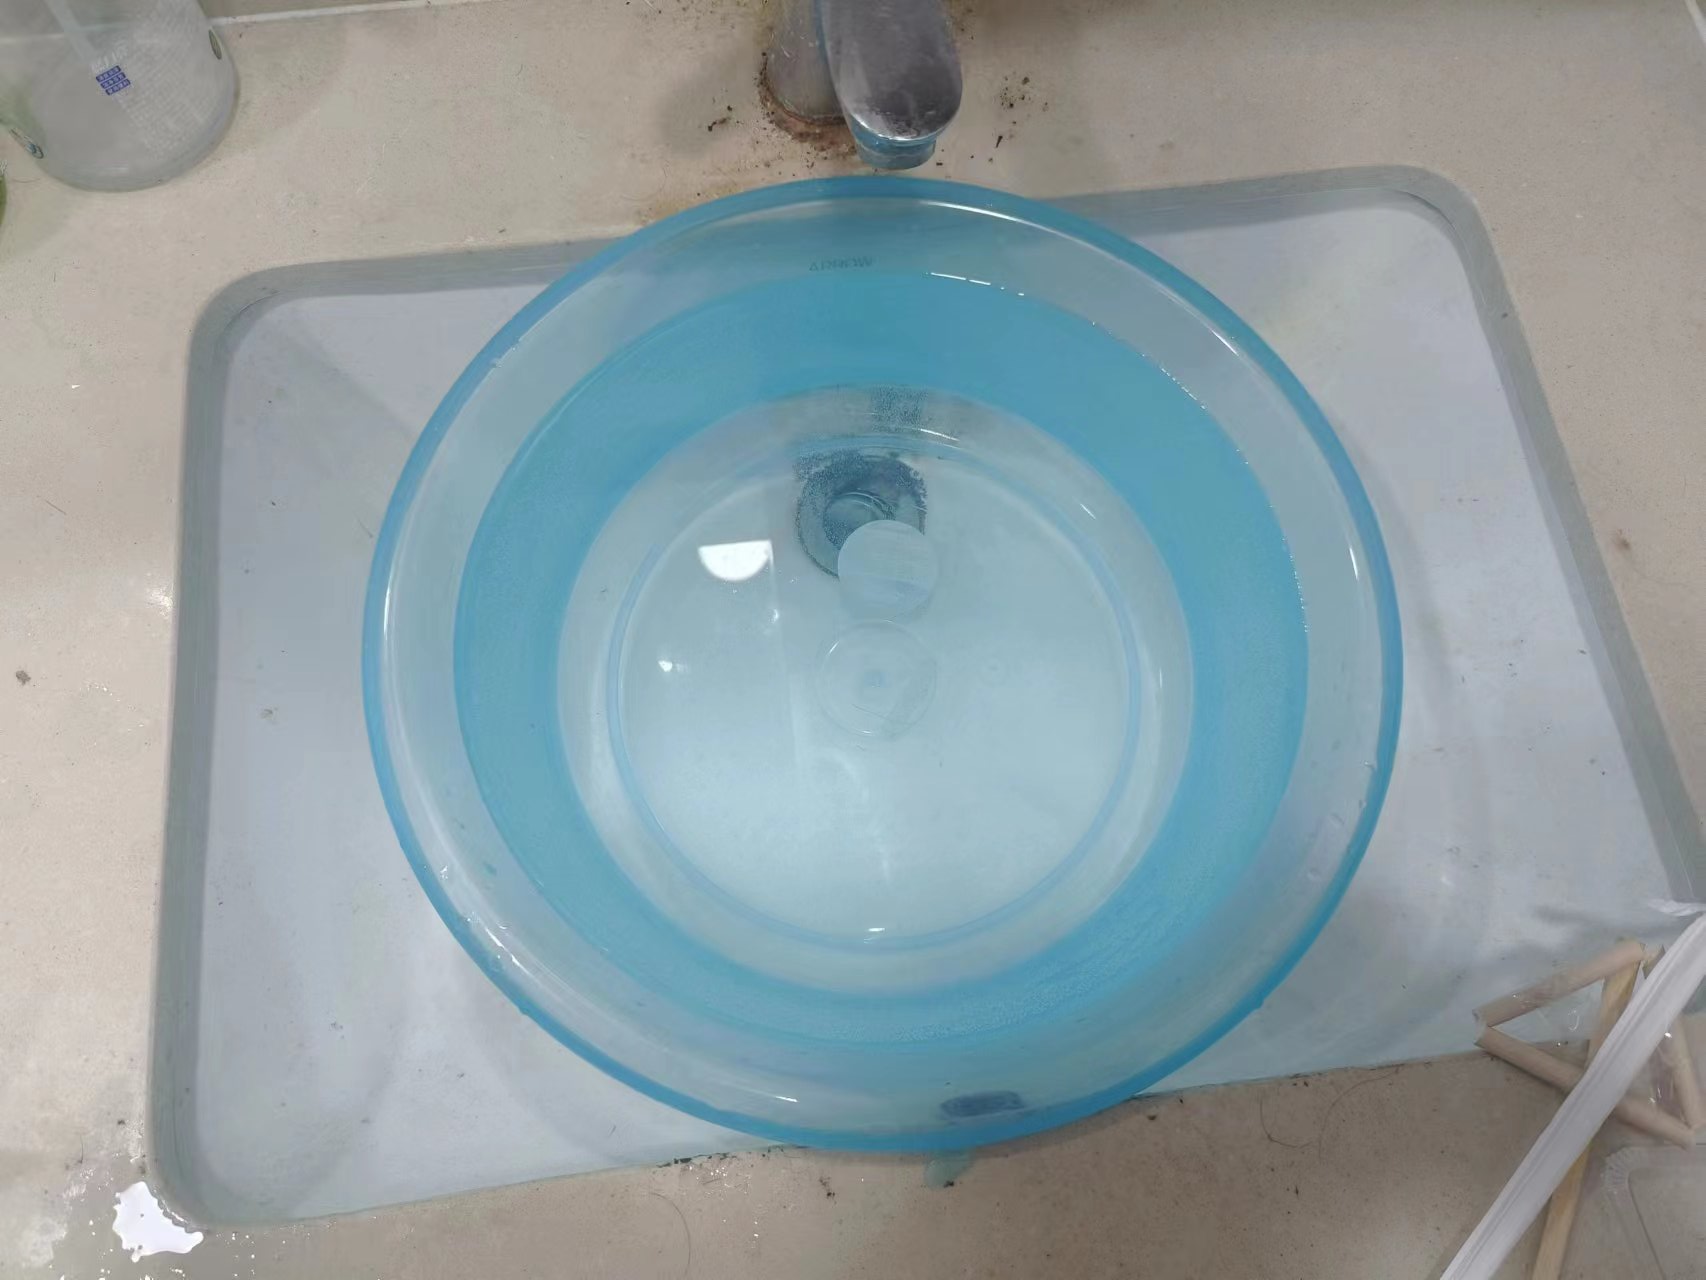
\includegraphics[scale=0.15]{9.png}
    \caption{水盆}
    \label{4}
\end{figure}


\subsection{实验内容与结果}

用手转动木棒,通过高速摄像机拍摄的照片,逐帧观察,数出转了多少圈,进而推测出角速度。由于手转动木棒角速度可能不太均匀,因此我们取一段时间 (大约 $0.5\text{s}$) 的平均值作为近似值。

由于在固定吸管面积的情况下,流量 $Q$ 正比于速度 $v$ ,我们只需知道 $v$ 即可用来反映流量 $Q$ 的情况。由于实际流量信息难以测量,速度也难以测量。因此我们采用定性分析的方法进行试验,我们通过肉眼观察出水的多少,来间接地定性衡量流量的大小。

为了使得旋转过程中吸管的角速度尽可能均匀且浸入深度不发生改变,木棒插在盆底的一个瓶盖 (用502黏在了盆底) 上,使得旋转过程中可以保证浸入水底的部分的深度不会发生改变。同时,通过改变垫的瓶盖的数量,我们可以改变吸管的浸入深度。


\subsubsection{截止角速度的估算}

用一只手在放在出水口附近判断是否有出水,从 $0$ 开始,逐渐加快角速度,直到有水流出为止。记录下此时的角速度,即为截止角速度。由于角速度可能不太均匀,因此我们取一段时间 (大约 $0.5\text{s}$) 的平均值作为近似值。同时,我们测多组,取平均来减小误差。

由公式, $v_l = \sqrt{\frac{1}{2}\omega^2 d^2 - gh}$ 。所以出水的必要条件是 $\omega > \frac{\sqrt{2gh}}{d} $ 。在这个估算实验中,测得设备 $h = 4\text{cm}$ , $H = 8\text{cm}$ , $2d = 9cm$ 。简单起见,取 $g = 9.8 \text{m}\cdot\text{s}^{-2}$ 。计算可得截止角速度 $\omega = 19.68 \text{rad} \cdot \text{s}^{-1} $ 。换算为截止频率 $f = \frac{\omega}{2\pi} = 3.13 \text{Hz} $ 。

实际测量截止角速度如下表:

\begin{table}[htbp]
    \centering
    \caption{截止角速度数据记录表}
    \label{table1}
    \renewcommand\arraystretch{1.5}
    \tabcolsep = 1cm
    \begin{tabular}{|c|c|c|}
        \hline
        数据组数 & $0.5\text{s}$ 内转过角度($\text{°}$)  & 截止转速 ($\text{Hz}$) \\
        \hline
        1 & 600 & 3.33 \\
        \hline
        2 & 590 & 3.28 \\
        \hline
        3 & 550 & 3.06 \\ 
        \hline
        4 & 630 & 3.50 \\
        \hline
        5 & 690 & 3.83 \\
        \hline
        6 & 530 & 2.94 \\
        \hline
        7 & 660 & 3.67 \\
        \hline
        8 & 730 & 4.06 \\
        \hline
    \end{tabular}
\end{table}

计算得平均截止频率 $\bar{f} = 3.51 \pm 0.43 \text{Hz}$ 。与理论值 $f = 3.13 \text{Hz}$ 相差不大,相对误差 $\delta_f = 12\%$ 。

\subsubsection{流量与露出水面的高度的关系}

对于同一套装置,通过改变垫在盆底的瓶盖(或其他障碍物)的数量来改变露出水面的高度 $h$ 。

首先,定性分析。当水面上高度 $h$ 变高,由公式可知, $v$ 会下降,因此流量会变低。我们选取了不同的高度,进行了定性的实验。观察到如下的现象:   当角速度相同的时候,露出的高度越高,出水量逐渐减小。如果初始角速度较慢,则可能在露出到一定程度的时候不再出水。该现象与我们的公式 $v_l = \sqrt{\frac{1}{2}\omega^2 d^2 - gh} $ 基本一致。

为了尽可能定量的反应出流量与露出水面高度的关系,我们用截止频率来反映流量的大小。我们认为,截止频率越低,在相同角速度下,流量越大。测量方法与之前一致,用 $0.5\text{s}$ 内转过的角度来估算平均角速度,从 $0$ 开始,逐渐加快角速度,直到有水流出为止。我们依然采用和之前一样的装置,即 $H = 8\text{cm}$ , $2d = 9cm$。不同的是,我们改变了浸入的深度(露出的深度),其分别为 $h = 1\text{cm}, 4\text{cm} , 7.5\text{cm}$ 。我们测量得到了以下的表格:

\begin{table}[htbp]
    \centering
    \caption{截止转速与露出高度数据记录表}
    \label{table2}
    \renewcommand\arraystretch{1.5}
    \tabcolsep = 1cm
    \begin{tabular}{|c|c|c|c|}
        \hline
        数据组数 & 露出高度 $h$ ($\text{cm}$) & $0.5\text{s}$ 内转过角度($\text{°}$)  & 截止转速 ($\text{Hz}$) \\
        \hline
        1 & 4 & 600 & 3.33 \\
        \hline
        2 & 4 & 590 & 3.28 \\
        \hline
        3 & 4 & 690 & 3.83 \\
        \hline
        4 & 4 & 660 & 3.67 \\
        \hline
        5 & 1 & 390 & 2.16 \\
        \hline
        6 & 1 & 300 & 1.67 \\
        \hline
        7 & 1 & 340 & 1.89 \\
        \hline
        8 & 1 & 270 & 1.50 \\
        \hline
        9 & 7.5 & 880 & 4.89 \\
        \hline
        10 & 7.5 & 750 & 4.17 \\
        \hline
        11 & 7.5 & 830 & 4.63 \\
        \hline
        12 & 7.5 & 820 & 4.56 \\
        \hline
    \end{tabular}
\end{table}

由上表,可以定性地看出,截止频率随露出高度的变大而变大。因此,露出水面高度越高,流量也越小。同时,我们通过计算可以得到,截止频率平均为 $f_1 = 1.80 \pm 0.24 \text{Hz} $ , $f_4 = 3.51 \pm 0.43 \text{Hz}$ , $f_{7.5} = 4.67 \pm 0.35 \text{Hz}$ 。

再定量分析 $f$ 与 $\sqrt{h}$ 的关系。注意到: 

$$
\begin{aligned}
    \frac{f_1}{\sqrt{h_1}} &= 18.0 \ \text{s}^{-1} \text{m}^{-0.5} \\
    \frac{f_4}{\sqrt{h_4}} &= 17.6 \ \text{s}^{-1} \text{m}^{-0.5} \\
    \frac{f_{7.5}}{\sqrt{h_{7.5}}} &= 17.1 \ \text{s}^{-1} \text{m}^{-0.5} \\
\end{aligned}
$$

容易看出, $\frac{f} {\sqrt{h}}$ 近似为常数,可以认为 $f \propto \sqrt{h}$ 。而这也与我们的公式 $f = \frac{\omega}{2\pi} = \frac{\sqrt{2gh}}{2\pi d}$ 基本一致。

\subsubsection{流量与三角形底边长度的关系}

类似之前,我们用截止频率来反映流量的大小,即认为截止频率越低,在相同角速度下,流量越大。

对于同一套装置,通过改变三角形底边长度 $2d$ 来改变流量 $Q$ 。我们不能再使用和以前一样的装置,而是用新的装置,改变底边吸管的长度,增长斜边吸管的长度,使得 $H = 8\text{cm}$ 和 $h=4\text{cm}$ 不变的情况下,仅改变了 $d$ 。

我们先定性分析。当 $d$ 变小的时候,由公式可知, $v$ 会下降,因此流量会变低。事实上,我们不仅观察到了其他条件不变在 $d$ 减小的时候,出水量会变少。当我们选取 $2d = 1\text{cm}$ ,即 $d = 0.5\text{cm}$ 的时候,我们发现,即使转速很快,也不会出水。通过摄像机估算,最高时候的转速达到了 $20\text{Hz}$ ,而根据公式,截止频率达到了 $28\text{Hz}$ ,因此应当无法出水,实际符合理论。

通过测量不同的 $d$ 时的数据,我们得到了以下的表格:

\begin{table}[htbp]
    \centering
    \caption{截止转速与底边长度数据记录表}
    \label{table3}
    \renewcommand\arraystretch{1.5}
    \tabcolsep = 1cm
    \begin{tabular}{|c|c|c|c|}
        \hline
        数据组数 & 底边长度 $2d$ ($\text{cm}$) & $0.5\text{s}$ 内转过角度($\text{°}$)  & 截止转速 ($\text{Hz}$) \\
        \hline
        1 & 9 & 600 & 3.33 \\
        \hline
        2 & 9 & 590 & 3.28 \\
        \hline
        3 & 9 & 690 & 3.83 \\
        \hline
        4 & 9 & 660 & 3.67 \\
        \hline
        5 & 12 & 450 & 2.50 \\ 
        \hline
        6 & 12 & 410 & 2.28 \\
        \hline
        7 & 12 & 500 & 2.78 \\
        \hline
        8 & 12 & 510 & 2.83 \\
        \hline
        9 & 4  & 1500 & 7.78 \\
        \hline
        10 & 4 & 1450 & 7.56 \\
        \hline
        11 & 4 & 1250 & 6.50 \\
        \hline
        12 & 4 & 1360 & 7.11 \\
        \hline
    \end{tabular}
\end{table}

由上表,可以定性地看出,截止频率随底边长度的变小而增大。因此,底边长度越小,流量也越小。同时,我们通过计算可以得到,截止频率平均为 $f_{12} = 2.60 \pm 0.22 \text{Hz} $ , $f_9 = 3.51 \pm 0.43 \text{Hz}$ , $f_{4} = 7.24 \pm 0.59 \text{Hz}$

再定量分析 $f$ 与 $d$ 的关系。注意到:

$$
\begin{aligned}
    {f_4}{d_4} &= 15.2 \ \text{s}^{-1} \text{cm} \\
    {f_9}{d_9} &= 15.9 \ \text{s}^{-1} \text{cm} \\
    {f_{12}}{d_{12}} &= 14.5 \ \text{s}^{-1} \text{cm} \\
\end{aligned}
$$

容易看出, $f \cdot d$ 近似为常数,可以认为 $f \propto d^{-1}$ 。而这也与我们的公式 $f = \frac{\omega}{2\pi} = \frac{\sqrt{2gh}}{2\pi d}$ 基本一致。


\subsection{实验结论}

本次实验,我们定量的分析了最低出水的截止频率与几何参数之间的关系,以及定性的给出了出水量与几何参数之间的关系。同时,我们也通过简化的理论模型,求出了理想情况下,出射水流的速度和几何参数的关系。

在理想情况下,出射速度满足 $v_l = \sqrt{\frac{1}{2}\omega^2 d^2 - gh}$ 。在实验中,我们通过测量截止频率来反映出射速度的大小。在实验中,我们发现,截止频率与 $\sqrt{h}$ 近似成正比,与 $d$ 近似成反比。这与理论模型的预测基本一致。在定性分析部分,我们发现当仅仅增大露出水面的高度时,出水量会减小;当仅仅增大三角形底边的长度时,出水量会增大。这也与理论模型的预测基本一致。

\subsection{误差分析与局限性}

在本次实验中,实测数据与理论值的在数量级上基本正确,且可以定性的解释一些现象,以及部分定量的求出一些关系,但是依然存在不小的误差。

首先,在理论模型上:  1. 我们做出了过分的简化,比如说认为水盆无限大,且吸管面积足够小,但实际上水盆面积有限,在实验开始一段时间后,会有部分液体被抽走,会导致水面下降,物体露出水面的高度变高,可能给实验引入误差。 2. 在计算水的压强时,我们认为水是无粘性的流体,但实际上水存在粘性,水和水之间,水和吸管之间都存在摩擦,而这又会进一步地引入误差。 3.由于买不到精密控制的仪器,吸管转动完全由手来控制,我们用 $0.5\text{s}$ 内转过的角度来估算平均角速度,但手并不稳定,因此角速度可能不太均匀,这也会引入误差。

我们的实验设计也存在一定的局限性:  1. 在本实验的定性部分中,我们不能直接测量出流量的大小,而是通过肉眼观察出水的多少,定性衡量水流的大小,这固然存在一定的局限性。 2. 在我们的部分定量部分,我们是使用旋转出水时的最低截止频率来间接反映流量的大小,认为在相同角速度下,若截止频率越低,则流量越大。这种间接衡量法在转动频率远大于截止频率时不一定适用。 3. 摄像机的帧率有限,每一帧的图像也比较模糊,我们对于具体的角度的衡量只能精确到 $10°$ ,这也会引入误差。

总之,由于设备过于简陋,本次实验的效果不是非常好,我们也未能完全验证具体出射速度的理论公式。如果能配备更好的高速摄像机,以及能够精准控制转速的电动机,实验的效果会有质的飞跃。

\end{document}
